\chapter{Introduzione}
In questa tesi andremo ad analizzare l'algoritmo di Boyer-Myrvold per “planarity testing”. Come introduzione all'argomento vi presento il seguente problema.
\begin{problema}[Problema delle 3 case]\label{problemaCase}
    Consideriamo 3 case, ognuna di esse ha necessità di essere allacciata a 3 risorse (acqua, luce e gas). È possile collegare ogni casa a ciascuna delle tre risorse senza creare intersezioni?
    \begin{figure}[H]
        \centering
        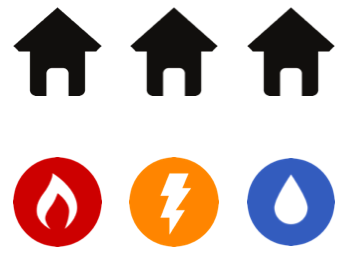
\includegraphics[scale=0.4]{img/3case.png}
        \caption{problema delle 3 case}
    \end{figure}
    \noindent Inizialmente si potrebbe ingenuamente cominciare a disegnare i collegamenti nella speranza di trovare una soluzione valida. Tuttavia, come dimostreremo nel lemma \(\ref{k5k33nonplanari}\), è impossibile evitare le intersezioni.
\end{problema}
Un interessante approccio alla risoluzione di questo quesito è quello di trasfrormarlo in un problema di planarity testing, per farlo avremo bisogno di una formulazione matematica di esso.
Le nozioni di cui ci serviremo furono pubblicate per la pirma volta nel 1736 da Leonhard Euler (1707~-~1783) all'interno dell'articolo “\textit{Solutio problematis ad geometriam situs pertinentis}\cite{ponti}”. In questo documento Eulero dimostrò la non esistenza della soluzione al problema dei sette ponti di Königsberg, per raggiungere tale obiettivo inventò quella che ad oggi chiamiamo teoria dei grafi.
\begin{definizione}[Grafo]
    Un grafo è una coppia \(G=(V,E)\) dove:
    \begin{itemize}
        \item \(V\) è un insieme di nodi (\textbf{vertex});
        \item \(E\) è un insieme di coppie di nodi \((u,v),\;u,v\in V\) dette archi o lati (\textbf{edge}); se un grafo è orientato avremmo che le coppie \(<u,v>\in E\) saranno ordinate (in questo documento assumeremo sempre \(G\) non orientato).
    \end{itemize}
\end{definizione}
\begin{definizione}[Grafo planare]\label{grafo-planare}
    Un grafo \(G\) si dice planare se può essere rappresentato nel piano evitando che gli archi si intersechino (se non negli endpoint).
\end{definizione}
Sfruttando queste nozioni possiamo ora dare una formulazione formale al problema delle case. Definiamo \(G\) grafo composto da 6 vertici (3 case e 3 risorse), ogni vertice “casa” sarà adiacente a ciascuno dei tre vertici “risorse”. La planarità di \(G\) corrisponderà invece alla richiesta di evitare le intersezioni fra le “linee”.

Nonostante la definizione di questo tipo di quesiti sia molto semplice, non sempre le soluzioni risutano banali. Lo studio di algoritmi efficienti per il “\textit{planarity testing}”  è stato infatti affrontato da molteplici matematici nel corso del 1900 e dei primi anni 2000.\\
Il primo algoritmo funzionante in tempo lineare fu “\textit{l'algoritmo di Hopcroft e Tarjan}\cite{Hopcroft}” pubblicato nel 1974. Esso si limitava però a fornire in output un valore booleano senza “disegnare” una reale immersione planare del grafo.
\begin{definizione}[Immersione planare]
    Dato un grafo \(G\), definiamo \(\psi : (V,E) \to \mathbb{R}^2\) la funzione che mappa i vertici di \(G\) nel piano e gli archi di \(G\) in curve continue che si intersecano solamente negli endpoint. Allora \(G^\psi \doteq \psi(G)\) è chiamata immersione planare di \(G\).
\end{definizione}
Solamente 30 anni dopo, grazie alla pubblicazione di John M. Boyer e Wendy J. Myrvold “\textit{Simplified \(O(n)\) Planarity by Edge Addition}\cite{main_article}”, è stato scoperto il primo algoritmo lineare in grado di resituire, se \(G\) planare, una sua immersione mentre, se \(G\) non planare, un sottografo di Kuratowski contenuto in esso. Dimostreremo infatti nel teorema \(\ref{Kuratowski}\) che un grafo \(G\) è non planare se e solo se contiene un sottografo di Kuratowski.
\\ In questo documento analizzeremo l'algoritmo di Boyer-Myrvold, le basi teoriche su cui è fondato, la sua complessità e le sue applicazioni.